\documentclass[11pt]{article}
\usepackage{amsfonts,amsmath,amssymb,amsthm}
\usepackage{array}
\usepackage{bm}
\usepackage{commath}
\usepackage{enumitem}
\usepackage{fancyhdr,fancyvrb}
\usepackage[letterpaper,text={7in,9in},centering]{geometry}
\usepackage[pdftex]{graphicx}
\usepackage[lofdepth,lotdepth]{subfig}
\usepackage{ifthen}
\usepackage{mathrsfs}
\usepackage{multicol}
\usepackage{pifont}
\usepackage{sectsty}
\usepackage{setspace}
\usepackage{stackrel}
\usepackage{stmaryrd}
\usepackage{tensor}
\usepackage{xspace}
\usepackage{natbib}
\usepackage{algorithm}
\usepackage{algpseudocode}

\pagestyle{fancy}
\fancyhead[RO]{Edward Gan \& Max Wang}

\sectionfont{\large}
\subsectionfont{\normalsize}

\newcommand{\Sequitur}{\textsc{Sequitur}\xspace}

\begin{document}
\bibliographystyle{plain}

\title{Squint: Lossy Hierarchical Compression on Symbol Streams}
\author{Edward Gan \& Max Wang}
\date{December 11, 2012}
\maketitle

\begin{abstract}
Grammar-based compression schemes like \Sequitur exploit repeated structures
in streams of symbolic data to achieve good compression ratios.
We develop a set of algorithms for improving upon Grammar-based compression 
schemes by allowing some loss in the compression. Although precise 
subsequences might be altered, in return we can simplify 
the grammars produced to obtain better ratios while still preserving
important syntatic patterns at both the micro and macro level.
\end{abstract}

\section{Introduction and Goals}
Many sources of data exhibit natural hierarchical structure. For instance,
english text often can be grouped well into sections, paragraphs, sentences, ...
all the way down to words and phonemes. Music too, consists of repeated motifs,
phrases, themes, and so on. Finally, computer code is so hierarchical that its
syntax can usually be put in BNF. This allows grammar-based compression schemes
to build up Context Free Grammars (CFGs) and achieve very good compression
ratios.

Taking a step back, in the image compression world there are both lossless and
lossy compression schemes. In certain situations, such as for low-pixel count
logos, one could use a lossless image compression scheme. In other situations
however, such as for textures and some photographs, the exact pixel values
are almost irrelevant compared to the overall gradients, colors, and structures
in the image, and one could use a lossy compression scheme like jpeg.

We believe it is valuable to bring some of the attitudes prevalent in image/
video compression to the world of hierarchical text compression. Better
compression ratios for text are possible. 

It may seem strange to allow a string such as "mind" to be lossily 
corrupted into ``rind'', but if one is more interested in recurrent 
structure in the text than in its precise meaning, these changes 
aren't important. For instance, if one is looking at a text in a foreign
language, one is more likely to pick up the texture, the repeated sounds,
some phrases that come up and the breaks between larger scale sections.
A change in a single letter probably wouldn't be noticed. Similarly,
when skimming through huge files, perhaps execution logs, one usually
first starts looking for patterns or things that stand out. Lorem ipsum
is a perfect example of a piece of ``text'' whose value lies in its texture
and sentence/paragraph structure, and we will come back to it again.

In this paper we develop 2 algorithms and implement a system for lossily
compressing text while preserving its hierarchical structures. The goal
was to preserve the feel of a text at both micro and macro levels. 
Since grammar-based compression schemes were designed to capture
these structures, we built
Music Final Composition: Dec 10
our system on top of the existing \Sequitur grammar inference algorithm. 
Starting with the CFG generated by a lossless grammar
inference algorithm, we repeatedly simplify it, throwing out details
along the way to emphasize repetitions. Our main contribution lies in the
development of 2 algorithms for ``simplifying'' CFG grammars while 
preserving their structure.

\section{Background}

TODO

\subsection{Grammar Compression}

TODO

\subsection{Lossy Compression}

TODO

Jpeg, Mpeg: using parts of previous frame to encode next frame, 
Fractal: Using self-similarity to encode

\section{Lossifier Algorithms}

\subsection{Motivation}

The scope of what we shall call a \emph{lossifier} algorithm is to take
an admissible CFG and simplify it. The output CFG should be smaller
than the input CFG but generate a string which preserves the
structure in the original string as much as possible. 

Building off the ideas in jpeg compression discussed
earlier, one idea for simplifying data is to look at a part
of the data and try to match it as closely as possible with an
existing set of primitives. In particular, just as with Mpeg and
fractal compression, to approximate one part of the grammar
we can use \emph{other parts of the grammar}. This is the seed for
both of our algorithms. Given a rule $S \rightarrow rhs$, we will
try to replace occurences of $S$ with other similar variables.

For example, consider the grammars in figure \ref{sred}.

\begin{figure}[t]
\centering
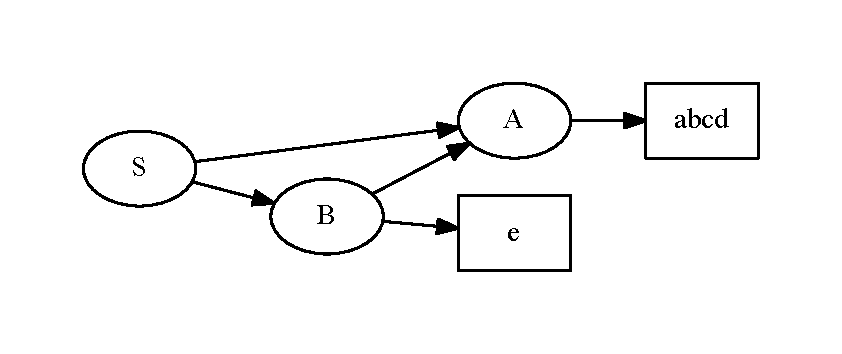
\includegraphics[scale=0.6]{sred1.pdf}
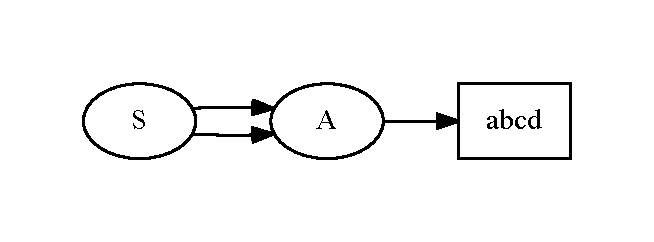
\includegraphics[scale=0.6]{sred2.pdf}
\caption{Grammar Simplification Example}
\label{sred}
\end{figure}

To simplify the grammar, it would make sense to replace B with A, since
they form two almost identical halves of S and are similar.

\subsection{Pair-Similarity}

To define whether two variables are \emph{similar}, we can look at their
expansions. Let $expand(rhs)$ denote the string of terminal symbols we get
when we recursively substitute all of the variables inside $rhs$. Then
$V_1 \rightarrow rhs_1$ and $V_2 \rightarrow rhs_2$ are similar when

$$\frac{levenshtein(expand(rhs_1),expand(rhs_2))}
        {max(len(expand(rhs_1)),len(expand(rhs_2)))} < \epsilon$$.

where $levenshtein$ is the levenstein edit distance between two strings.
For convenience we can define.

$$lsim(s1,s2) = \frac{levenshtein(s1,s2)}{max(len(s1),len(s2))}$$

The first algorithm takes the idea of variable similarity and uses it
to simplify the grammar sequentially as much as possible.

\begin{algorithm}[h]
\caption{Similarity Lossifier Algorithm}
\label{sim_alg}
\begin{algorithmic}[1]
\Procedure{Lossify-Sim}{$g$} \Comment{Simplify grammar g}
  \While{there are similar variables to replace}
    \For{$var_1 \rightarrow rhs_1,\ var_2 \rightarrow rhs_2 \in g$}
      \State $str_{i} \gets expand(rhs_i)$
      \If{$lsim(str_{1},str_{2})<\epsilon$}
        \State replace the longer var with the smaller throughout $g$
        \State break
      \EndIf
    \EndFor
  \EndWhile
\EndProcedure
\end{algorithmic}
\end{algorithm}

\subsection{Clustering}

The previous algorithm updates the grammar sequentially, since each
variable replacement can have an effect on large parts of the grammar,
we will have to go through comparing all pairs again after the change.
An alternative algorithm would be to try to replace similar variables in
parallel. This would avoid many of the repeat pair-comparisons done in
\emph{Similarity}. In other words, the algorithm below puts 
similar variables
into equivalence class clusters, and then replaces each variable
in a cluster them with a representative
all at once each iteration.

\begin{algorithm}[h]
\caption{Cluster Lossifier Algorithm}
\label{cluster_alg}
\begin{algorithmic}[1]
\Procedure{Cluster-Sim}{$g$} \Comment{Simplify grammar g}
  \While{there are similar variables to replace}
    \State $clusters \gets ()$
    \For{$var_1 \rightarrow rhs_1 \in g$}
      \For{$c \in clusters$}
        \State $(var_2 \rightarrow rhs_2) \gets $ first variable in $c$
        \State $str_{i} \gets expand(rhs_i)$
        \If{$lsim(str_{1},str_{2})<\epsilon$}
          \State add $var_1$ to $c$
          \State break
        \EndIf
      \EndFor
      \If{$var_1$ hasn't been added to a cluster}
        \State Add $var_1$ to a new cluster in $clusters$
      \EndIf
    \EndFor
    \For{Cluster $c \in clusters$}
      \State replace all $var \in c$ with the smallest.
    \EndFor
  \EndWhile
\EndProcedure
\end{algorithmic}
\end{algorithm}

Both of the algorithms depend on the concept of the "smallest / smaller"
variable. We can define the size of a variable to be the length of
the expansion of its rhs. In this way, if we think of our CFG's as a DAG, then
variables higher up on the DAG will always have larger expansions than
those lower down, and thus will have a larger size. By always replacing
with the smallest variable, we avoid creating cyclic references in our CFG.
We will prove this fact in the next section.

\subsection{Runtime Estimates}
Given an input of length $n$, let $r$ be the number of rules generated
by Sequitur from the input. Let $R$ be the total number of variable
replacements we perform. For each replacement, we had to have searched though
up to all pairs of variables, and for each pair of variables expanding
them and calculating the levenshtein distance could take time linear in $n$.
Thus the runtime is $\boxed{O(R*r^2*n)}$. 

From the \Sequitur paper \cite{sequitur} we
know that the number of rules in the grammar generated by Sequitur
is between $O(\sqrt{n})$ and $O(n)$. Thus the worst case runtime on the similarity
algorithm is $\boxed{O(n^4)}$. This is because we could have up to $r$ replacements.
However, in practice we will see that the runtime is much better
than $O(n^4)$. This is because we found $r$ for our test data to be slightly sublinear
even for complicated english text, and we found that we didn't quite make a linear
number of replacements $R$ with respect to $r$.
so our optimistic runtime could be anywhere 
from $O(n^4)$ to $O(n^{2})$ depending on how $r$ grows.



The inner loops of the Cluster are similar to those of the Similarity algorithm.
We iterate the entire clustering and replacement procedure $C$ times. Going through
each variable-cluster pair takes up to $O(r^2)$ time and calculating the levenshtein
distance takes $O(n)$ time. The time taken to actually perform the replacements each
iteration is absorbed into the $O(r^2)$ term. So, again we have a runtime of
$\boxed{O(C*r^2*n)}$. The big gain over the similarity algorithm is that $C$ turns out
to be nearly constant, since there are very few huge chains of reductions that are
only possible after other reductions have been performed, an in fact we are able to 
perform a very large number of the remaining reductions each time we perform an iteration
of the clustering algorithm. Thus since $C$ is nearly constant, the optimistic runtime
could be anywhere from $O(n^3)$ to $O(n^2)$. 


CANT THINK OF PROOF OF NOLOOPS

\section{Implementation}
Overview

\subsection{Grammar Reductions}
What is their purpose? Why do we want them? What are they?

\subsection{Data Structures and Optimizations}
Grammar Data Structure
Cluster Data Structure
Invariants Maintained
Core utility methods??
Linked Lists vs Arrays, Caching Expansions, Strings vs Symbols for expansion, Native Levenshtein

\section{Results}
\subsection{Illustrative Examples}
It is useful to look at how the algorithms function on a small piece of
data with both plenty of hierarchical structure, and also some messiness
that most lossless compression schemes would not deal well with. Take
the string below, similar to what one might come across in a math
puzzle book.

\begin{verbatim}
123,124,123 + 321,323,321 = ???
124,123,123 + 321,3231,321 = ????
--
124,123,123 + 321,3231,321 = ????
123,124,123 + 321,323,321 = ????
\end{verbatim}

Disregarding its meaning, it consists of four very similar equations of the
form $a + b = ?$, and on a smaller scale each summand consists of
3 repetitions of approximately the same string of either $123,$ or $321,$.

When comparing grammars, we chose to define the \emph{size} of a grammar
as the sum of the lengths of the rhs's of the production rules.
Sequitur yields a relatively complicated inferred grammar with 13 rules and
a size of 51. Both the Similarity and Clustering Algorithms with $\epsilon = .4$
, yield the following grammar after reduction. It has 5 rules and is almost
half the size, at 30.

\begin{verbatim}
Grammar:
~[*] => ~[BC]--~[BC]?

~[AZ] => ~[A]3~[A]~[A] + ~[C]~[C]3~[C]1 = ???
~[A] => 12
~[BC] => ~[AZ]~[AZ]
~[C] => 32
-----------------------
Generated String:
1231212 + 32323321 = ???1231212 + 32323321 = ???--(cont.)
1231212 + 32323321 = ???1231212 + 32323321 = ????
\end{verbatim}


The lossifier algorithm reduced the string to a pair of
pairs of the same equations, where each equation consists of the
sum of triples of "12" or "32". Smaller discrepencies
in the numbers involved were dropped, while the filler
commas and linebreaks also ended
up being lost. Note that the structure described is easily
observable from the grammar generated.

\subsection{Similarity vs Clustering}
For most of our benchmark tests, we focused on two extreme kinds of data:
one with large amounts of repetition at all levels, and one with a word
and sentence level structure but with little obvious large-scale repetition.
One set of test data was constructed by repeating the same letter `a' n-times
but then adding some
texture to the data by changing 1/30 of the characters uniformly
at random to `*'. Call these test-cases \emph{rep-n}
Another set of test data was constructed from the first n characters of the
book of Genesis from the KJV. Call these test-cases \emph{gen-n}

For our first suite of tests, we compare the effectiveness of the
\emph{Similarity} and \emph{Cluster} algorithms. We might expect
Similarity to achieve better quality at the same compression ratio
since it updates the state of the grammar between each variable
replacement, on the other hand since it must update the grammar
it has the potential to run much more slowly than Cluster.

We don't report the running times for just \Sequitur since its linear
running time is negligible compared to our algorithms for all but the
smallest input data.

\subsubsection{Rep-n results}

Below are the results on running Sequitur and Cluster, without
the grammar reductions, on the rep-n datasets. Time is the wall clock
running as measured on a 2.26 Ghz Intel Core 2 Duo Macbook Pro.
Ratio is the relative size of the grammar produced compared with
Sequitur, where the size of the grammar is the sum of the lengths of the
rhs's of the rules. Levdistance is the levenshtein distance between
the output of the lossified grammar and the original input string, it
is a kind of measure of the fidelity of our algorithms but doesn't
take into account how well patterns were preserved. For the rep-n tests,
proportion is the proportion of the final string produced that was
`*'. The closer to 1/30~0.033, the more accurate the lossifier was
in recreating the original texture of the input.

The columns of the data are prefixed by S or T depending on whether
they are measurements for sequitur or cluster respectively.

\begin{table}[p]
\subfloat[$\epsilon = .4$]{
\begin{tabular}{l|l|l|l|l||l|l|l|l}
Dataset & S-T(ime) & S-R(atio) & S-L(evdistance) & S-P(roportion) & C-T & C-R & C-L & C-P \\
\hline
rep-100   & 0.006 & 18/34    & 0.713 & 0.07 & 0.002 & 20/34    & 0.535 & 0.04\\
rep-400   & 0.028 & 45/76    & 0.269 & 0.01 & 0.009 & 41/76    & 0.743 & 0.04\\
rep-1600  & 0.355 & 103/194  & 0.873 & 0.03 & 0.042 & 103/194  & 0.804 & 0.02\\
rep-6400  & 3.978 & 258/448  & 0.706 & 0.005& 0.203 & 256/448  & 0.869 & 0.50\\
rep-12800 & 44.63 & 604/1064 & 0.791 & 0.01 & 1.136 & 600/1064 & 0.856 & 0.01\\
rep-25600 & 135.0 & 900/1482 & 0.829 & 0.005& 2.906 & 898/1482 & 0.725 & 0.25\\
\end{tabular}
}

\subfloat[$\epsilon = .2$]{
\begin{tabular}{l|l|l|l|l||l|l|l|l}
Dataset & S-T(ime) & S-R(atio) & S-L(evdistance) & S-P(roportion) & C-T & C-R & C-L & C-P \\
\hline
rep-100   & 0.002 & 30/34    & 0.040 & 0.05 & 0.002 & 30/34    & 0.040 & 0.05\\
rep-400   & 0.019 & 60/76    & 0.035 & 0.02 & 0.009 & 60/76    & 0.035 & 0.02\\
rep-1600  & 0.350 & 123/194  & 0.355 & 0.03 & 0.055 & 123/194  & 0.206 & 0.01\\
rep-6400  & 3.942 & 280/448  & 0.387 & 0.08 & 0.295 & 274/448  & 0.543 & 0.09\\
rep-12800 & 42.21 & 638/1064 & 0.491 & 0.03 & 1.105 & 632/1064 & 0.457 & 0.01\\
rep-25600 & 124.5 & 922/1482 & 0.565 & 0.12 & 2.597 & 926/1482 & 0.437 & 0.007\\
\end{tabular}
}
\caption{rep-n Tests}
\end{table}

The compression ratios achieved for both algorithms are roughly equal for the same
value for $\epsilon$, so it is fair to compare the algorithms for the same $\epsilon$.


From plotting the data, we see that runtime of the algorithms are roughly polynomial
in the size of the data, so we can perform a linear regression on the log-log transform
of the data to find the exponents $\alpha$ for the runtime $r(n)=n^\alpha$ where $n$ is the
length of the input string. In the chart below, all of the linear regressions had
$R^2$ values of over $0.98$.

\begin{tabular}{l|l|l|l|l}
Data     & Sim: $\epsilon=.4$ & Sim: $\epsilon=.2$ & Clust: $\epsilon = .4$ & Clust: $\epsilon = .2$ \\
Exponent & $1.859$ & $2.026$ & $1.306$ & $1.305$
\end{tabular}


For both values of $\epsilon$, 
The clustering algorithm is nearly linear, while the similarity algorithm is roughly
quadratic. On this dataset, the leveshtein distances were similar for both algorithms
but fairly high since the length of the final string could change drastically.
The proportion of '*'s in the input was usually the right order of magnitude,
with both algorithms making big mistakes occassionally. In most cases,
the two algorithms maintained similarly acceptable fidelity levels in recreating
the texture of the original rep-n input file.

Setting higher values for $\epsilon$ had diminishing returns for compression
for larger and larger file sizes, at the cost of drastically lowering the fidelity
of the output. 

\subsubsection{Gen-n results}

Repeating the above tests on the \emph{gen-n} datasets yields the following:

\begin{table}[p]
\subfloat[$\epsilon = .4$]{
\begin{tabular}{l|l|l|l||l|l|l}
Dataset & S-T(ime) & S-R(atio) & S-L(evdistance) & C-T & C-R & C-L \\
\hline
gen-100   & 0.006 & 87/89    & 0.04 &0.006 & 87/89    & 0.04\\
gen-400   & 0.175 & 224/258  & 0.12 &0.069 & 219/258  & 0.19\\
gen-1600  & 4.863 & 539/697  & 0.31 &0.732 & 529/697  & 0.33\\
gen-6400  & 216.9 & 1740/2348& 0.41 &9.127 & 1694/2348& 0.43\\
gen-12800 & 1812  & 3296/4523& 0.40 &29.17 & 3181/4523& 0.44\\
gen-25600 & 12989 & 5823/8060& 0.43 &176.7 & 5540/8060& 0.50\\
\end{tabular}
}



\subfloat[$\epsilon = .2$]{
\begin{tabular}{l|l|l|l||l|l|l}
Dataset & S-T(ime) & S-R(atio) & S-L(evdistance) & C-T & C-R & C-L \\
\hline
gen-100   & 0.004 & 89/89    & 0.00 &0.002 & 89/89    & 0.00 \\
gen-400   & 0.085 & 245/258  & 0.03 &0.053 & 245/258  & 0.03 \\
gen-1600  & 1.292 & 664/697  & 0.03 &0.874 & 664/697  & 0.03 \\
gen-6400  & 73.83 & 2173/2348& 0.05 &14.02 & 2171/2348& 0.05\\
gen-12800 & 549.2 & 4197/4253& 0.05 &45.64 & 4186/4253& 0.05\\
gen-25600 & 3939  & 7405/8060& 0.06 &224.9 & 7374/8060& 0.06\\
\end{tabular}
}
\caption{gen-n}
\end{table}

Just as with the rep-n data, log-log regression tests yield the following
exponents for the runtime on the gen-n data.

\begin{tabular}{l|l|l|l|l}
Data     & Sim: $\epsilon=.4$ & Sim: $\epsilon=.2$ & Clust: $\epsilon = .4$ & Clust: $\epsilon = .2$ \\
Exponent & $2.629$ & $2.493$ & $1.814$ & $2.061$
\end{tabular}


Again, the two algorithms have almost identical compression ratios and
their fidelity is about the same both subjectively and based on levenshtein
distance.


INCLUDE SAMPLE TEXT


The runtimes are noticeably worse than for the rep-n dataset. The
similarity algorithm runs in roughly $n^{2.5}$ time while cluster
runs in roughly $n^2$ time. 


Changing epsilon in this case had a large effect on both the compression
ratio and the fidelity of the final output string.

\subsubsection{Summary}

Both of the algorithms were able to achieve great additional compression
ratios on top of \Sequitur of up to about 40 percent for the highly
structured rep-n data, and 30 percent for the more loosely structured
gen-n data without using the grammar reducer. The fidelity between
the original and lossified strings wasn't great as measured by
levenshtein distance, but the texture in both the rep-n and
gen-n datasets was preserved well. Decreasing the $\epsilon$ threshold
improved fidelity greatly for larger very structured data at little
cost to the compression ratio, but hurt the compression ratio
a lot for less structured data.

The differences between the two algorithms lie almost entirely in their
runtime. Both algorithms perform much worse on the less structued
gen-n data, we believe because simplifications are made more incrementally
and the grammar does not get dramatically simpler after a few iterations
of our algorithm like it does for the rep-n data.
Unfortunately the Similarity algorithm tends to consistently incur
an overhead of about $O(\sqrt{n})$ on top of the runtime for the
Cluster algorithm. Because of this we dismiss the Similarity algorithm
as unscalable and do not test it further.

\subsection{Grammar Reduction Impact}
Although the grammars generated by Sequitur are irreducible,
our lossifiers produce grammars which could potentially be
compressed further (losslessly) using Reduction Rules without
changing the output string. To test the cost and
effectiveness of applying reduction rules, we looked at the
rep-n and gen-n test cases again, this time focusing on the
clustering algorithm for $\epsilon = .2$. This time we give the ratio
on top of the simplified grammar produced by the clustering algorithm,
and the time taken to run just the reduction rules.

\begin{table}[p]
\subfloat[rep-n tests]{
\begin{tabular}{l|l|l}
Dataset & Time & Ratio \\
\hline
rep-100   & 0.008 & 29/30  \\
rep-400   & 0.028 & 56/60  \\
rep-1600  & 0.132 & 96/123 \\
rep-6400  & 1.145 & 153/186\\
rep-12800 & 19.43 & 403/632\\
\end{tabular}
}
\subfloat[gen-n tests]{
\begin{tabular}{l|l|l}
Dataset & Time & Ratio \\
\hline
gen-100   & 0.016 & 89/89\\
gen-400   & 0.126 & 245/245\\
gen-1600  & 4.833 & 660/664\\
gen-6400  & 308.7 & 2139/2171\\
\end{tabular}
}
\caption{Reducer Tests for $\epsilon = .2$}
\end{table}


When plotted on a log-log scale, the runtime for our straightforward 
implementation of the reduction
rules appears to be superpolynomial. While modest additional gains of about 30 percent
are possible for highly self-similar data, very few additional gains are
possible for more diverse datasets such as gen-n. This appears to be because
the only simplifications that are possible on diverse datasets don't lead to
the wide-ranging repetitive substitutions which allow reduction rules to be allowed.
The simplifications in gen-n tend to be more local.

Because we were unable to get reduction rules to scale to larger datasets,
we will not consider them further.


\subsection{Larger Tests}
Genesis-256000
Obfuscated C Code (looks really cool!)

\section{Conclusions}
\subsection{Summary of Results}
* General concept of simplifying grammars, two proposed algorithms
* reasonably efficient implementation with runtime better than expected
* compared algorithms, evaluated effectiveness of reducer
* looked at effect of epsilon

\subsection{Ratios and Fidelity}

* How useful are these algorithms??
* What is the ratio we get
* What kind of fidelity to we get

\subsection{Future Work}
* Better ways to set epsilon to maximize value / cost for different size and types
* Better ways to quantify preservation of hierarchies
* How to find near `self-similarities' that aren't captured by a rule
* Iterating lossify and reduce in a cycle

\nocite{*}

\bibliography{sources}

\end{document}
